% ======================================================================


% Sujet du document
% Informations importantes
%
%
% Prénom Nom
% H. Dube 2019
% ======================================================================
% Ce code rassemble les efforts d'étudiants de la faculté de génie  
% de l'université de Sherbrooke afin de faire un template LaTeX moderne
% dédié à l'écriture de rapport universitaire.
% Ce document est libre d'être utilisé et modifié.
% ======================================================================

% ----------------------------------------------------
% Initialisation
% ----------------------------------------------------
\documentclass{udes_rapport} % Voir udes_rapport.cls

\begin{document}
\selectlanguage{french}

% ----------------------------------------------------
% Configurer la page titre
% ----------------------------------------------------

% Information
\faculte{Génie}
\departement{génie électrique et génie informatique}
\app{1}{Éléments de statique et de dynamique}
\professeur{M.}
\etudiants{Hubert Dubé - dubh3401 \\ Marc Sirois - sirm2508\\ Gabriel Lavoie - lavg2007}
\dateRemise{4 septembre 2019}


% ======================================================================
\pagenumbering{roman} % met les numéros de pages en romain
% ----------------------------------------------------
% Page titre
% ----------------------------------------------------
\fairePageTitre{LOGO} % Options: [STD, LOGO]
\newpage

% ----------------------------------------------------
% Table des matières
% ----------------------------------------------------
\tableofcontents
\newpage


% ----------------------------------------------------
% Table des figures
% ----------------------------------------------------
\listoffigures
\newpage



% ======================================================================
% Document
% ======================================================================
\pagenumbering{arabic} % met des chiffres arabes
\setcounter{page}{1} % reset les numéros de pages
%%%%%%%%%%%%%%%%%%%%%%%%%%%%%%%%%%%%%%%%%%%%%%%%%%%%%%
%{Analyse du signal
%%%%%%%%%%%%%%%%%%%%%%%%%%%%%%%%%%%%%%%%%%%%%%%%%%%%%%
\section{Introduction}

\section{Cinématique}
\subsection{Mouvement de A dans le cas général}
Le positionnement de $\overrightarrow{OA}$ peut être exprimé par l'addition:
\begin{align}
	\overrightarrow{OA} = \overrightarrow{OB} + \overrightarrow{BA}	\\
	\overrightarrow{OA_x} = l_1 cos(\theta) + l_2 cos(\phi) 		\\
	\overrightarrow{OA_y} = l_1 sin(\theta) + l_2 sin(\phi)
\end{align}

la vitesse étant la dérivée de la position :
\begin{align}
\overrightarrow{V_A} = \frac{d\overrightarrow{OA}}{dt}	\\
\overrightarrow{V_Ax} = \frac{d\overrightarrow{OA_x}}{dt} = \frac{l_1 cos(\theta) + l_2 cos(\phi)}{dt}	\\
\overrightarrow{V_Ax} = -l_1 sin(\theta) \dot{\theta} -l_2 sin(\phi) \dot{\phi}\\
\overrightarrow{V_Ay} = \frac{d\overrightarrow{OA_y}}{dt} = \frac{l_1 sin(\theta) + l_2 sin(\phi)}{dt}	\\
\overrightarrow{V_Ax} = l_1 cos(\theta) \dot{\theta} -l_2 cos(\phi) \dot{\phi}\\
\end{align}

La même stratégie peut être utilisé pour obtenir l'accélération :
\begin{align}
\overrightarrow{a_A} = \frac{d\overrightarrow{V_A}}{dt}	\\
\overrightarrow{a_Ax} = \frac{d\overrightarrow{OA_x}}{dt} = \frac{l_1 cos(\theta) + l_2 cos(\phi)}{dt}	\\
\end{align}

\subsection{Mouvement horizontal de A}

\noindent\begin{minipage}{\textwidth} 
\begin{minipage}{0.5\textwidth}
  \centering
  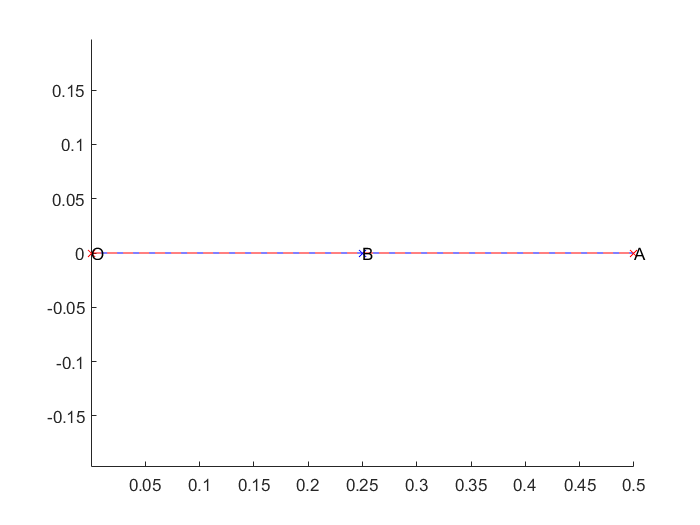
\includegraphics[width=.75\linewidth]{pos_hori_0}
  \captionof{subfigure}{Position initiale}
  \label{pos_hori:position_horizontal_initiale}
\end{minipage}%
\begin{minipage}{0.5\textwidth}
  \centering 
  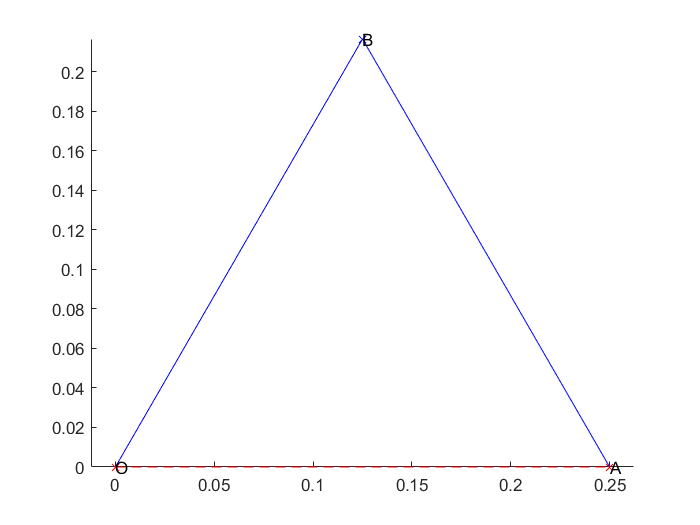
\includegraphics[width=.75\linewidth]{pos_hori_pi3} 
  \captionof{subfigure}{Position finale} 
  \label{pos_hori:position_horizontal_finale} 
\end{minipage} 
\captionof{figure}{Position du mouvement horizontale} 
\label{pos_hori} 
\end{minipage}


\begin{center}
	\centering
	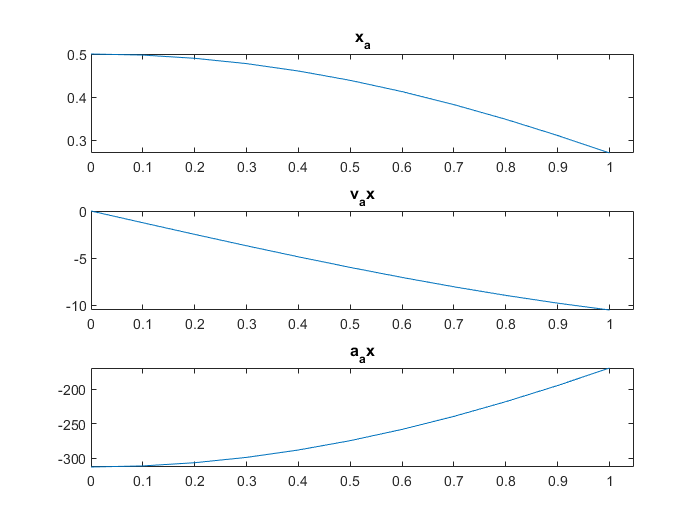
\includegraphics[width=0.7\textwidth]{theta_hori}
	\captionof{figure}{Composantes en fonction de $\protect\theta$}
	\label{composantes_horizontale_theta}
\end{center}

\subsection{Mouvement vertical de A}

\noindent\begin{minipage}{\textwidth} 
\begin{minipage}{0.5\textwidth}
  \centering
  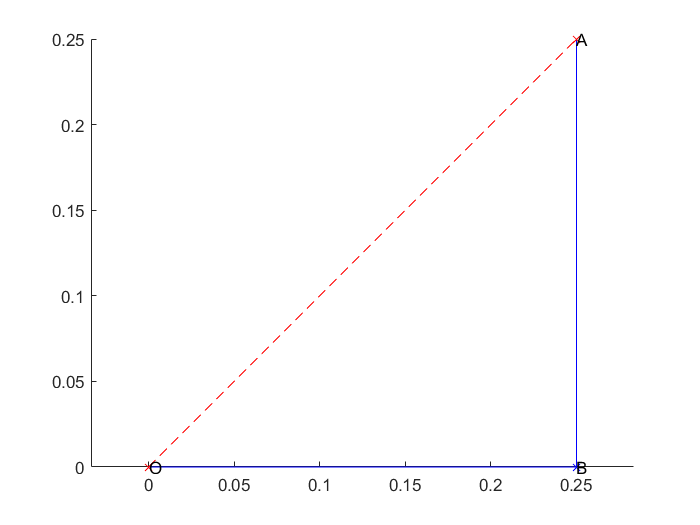
\includegraphics[width=.75\linewidth]{pos_vert_0}
  \captionof{subfigure}{Position initiale}
  \label{pos_vert:position_verticale_initiale}
\end{minipage}%
\begin{minipage}{0.5\textwidth}
  \centering 
  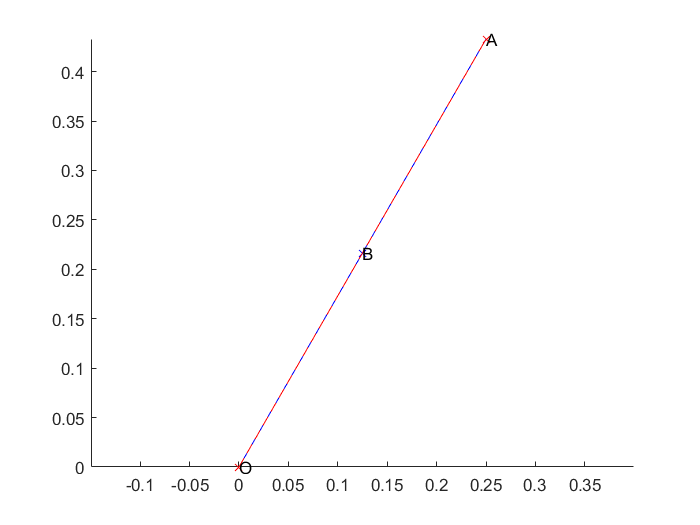
\includegraphics[width=.75\linewidth]{pos_vert_pi3} 
  \captionof{subfigure}{Position finale} 
  \label{pos_vert:position_verticale_finale} 
\end{minipage} 
\captionof{figure}{Position du mouvement vertical} 
\label{pos_vert} 
\end{minipage}

\begin{center}
	\centering
	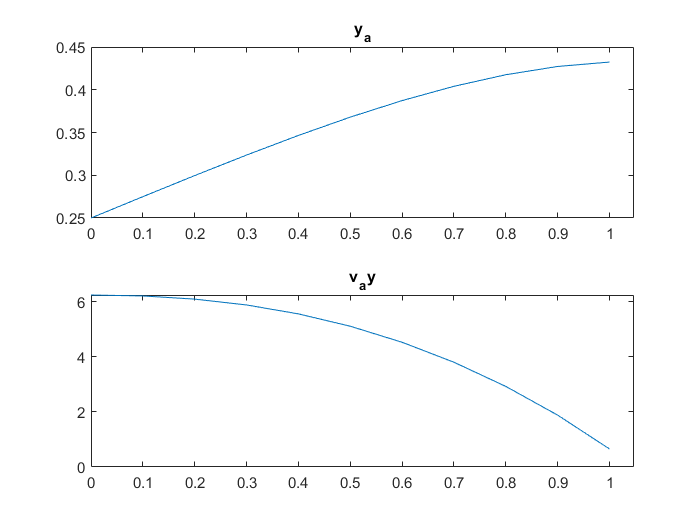
\includegraphics[width=0.7\textwidth]{theta_vert}
	\captionof{figure}{Composantes en fonction de $\protect\theta$}
	\label{composantes_verticale_theta}
\end{center}
\subsection{Analyse avec Matlab}



\section{Statique et dynamique}
\subsection{Statique}
\begin{center}
	\centering
	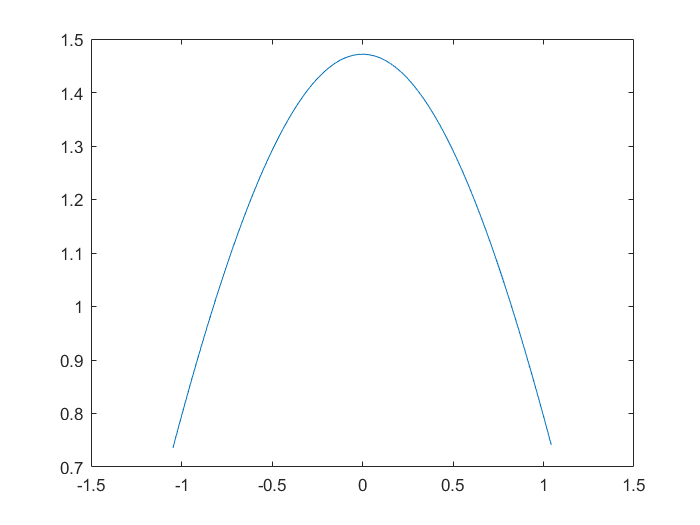
\includegraphics[width=0.7\textwidth]{couple_stat}
	\captionof{figure}{couple statique en fonction de $\protect\theta$}
	\label{couple_statique}
\end{center}
\subsection{Dynamique}
\begin{center}
	\centering
	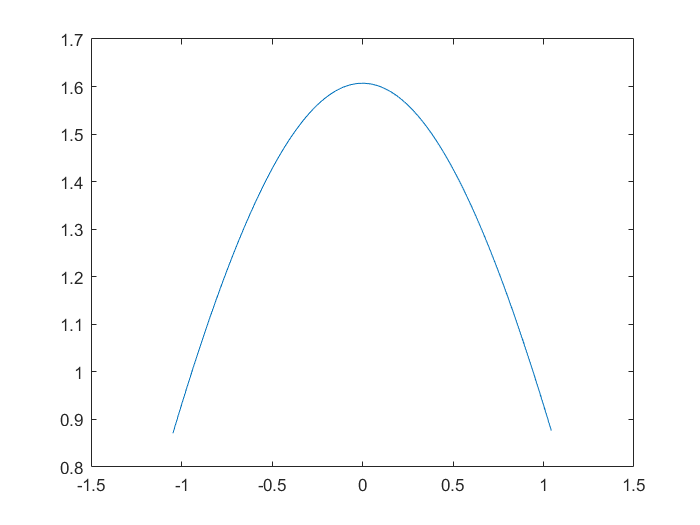
\includegraphics[width=0.7\textwidth]{couple_dyn}
	\captionof{figure}{couple dynamique en fonction de $\protect\theta$}
	\label{couple_dynamique}
\end{center}
\subsection{Analyse avec Matlab}

\section{Conclusion}

\begin{comment}
\begin{center}
	\centering
	\includegraphics[width=0.7\textwidth]{puissance}
	\captionof{figure}{Spectre de puissance d'une onde de 1kHz}
	\label{puissance}
\end{center}


\section{Filtres FIR}
\noindent\begin{minipage}{\textwidth} 
\begin{minipage}{0.5\textwidth}
  \centering
  \includegraphics[width=.75\linewidth]{ampFIR}
  \captionof{subfigure}{Amplitude}
  \label{FIR:ampFIR}
\end{minipage}%
\begin{minipage}{0.5\textwidth}
  \centering 
  \includegraphics[width=.75\linewidth]{phaseCute} 
  \captionof{subfigure}{Phase} 
  \label{FIR:phaseFIR} 
\end{minipage} 
\captionof{figure}{Filtre IIR} 
\label{FIR} 
\end{minipage}
\end{comment}

\end{document}












